% Metódy inžinierskej práce

\documentclass[10pt,twoside,slovak,a4paper]{article}

\usepackage[slovak]{babel}
%\usepackage[T1]{fontenc}
\usepackage[T1]{fontenc} % lepšia sadzba písmena Ľ než v T1
\usepackage[utf8]{inputenc}
\usepackage{graphicx}
\usepackage{url} % príkaz \url na formátovanie URL
\usepackage{hyperref} % odkazy v texte budú aktívne (pri niektorých triedach dokumentov spôsobuje posun textu)
\usepackage{todonotes}
\usepackage{cite}
% \usepackage{fancyhdr}
\usepackage{wrapfig}
\usepackage{stfloats}
%\usepackage{times}

% \pagestyle{fancy}
% \fancyhead{}



\title{Je odporúčací systém Netflix-u problém ?\thanks{Semestrálny projekt v predmete Metódy inžinierskej práce, ak. rok 2024/2025, vedenie: Mgr. Yevheniia Kataieva, PhD.}}

\author{Adam Glogovský\\[2pt]
	{\small Slovenská technická univerzita v Bratislave}\\
	{\small Fakulta informatiky a informačných technológií}\\
	{\small \texttt{xglogovsky@stuba.sk}}}

\date{\small 5. október 2024} 


\begin{document}

\maketitle
\begin{abstract}
	Touto prácou by som chcel poukázať na to, ako Netflix ako firma spracúva užívateľské informácie a či je to správne. Na začiatku tejto práce objasním problematiku všeobecných odporúčacích systémov. Potom ukážem kde Netflix posiela užívateľské informácie. Ako ich spracúva a ako podľa nich dokáže nám užívateľom spríjemniť fungovanie na platforme. Ak nám to zvyšuje zážitok z používania tejto platformy, čo to teda tú platformu stojí a či je to vo výsledku pre danú platformu efektívne a finančne prospešné. Taktiež sa pokúsim čo naviac priblížiť samotné spracovanie týchto údajov a poukážem na to, či je správne daným spôsobom spracúvať tieto informácie.\cite{amatriain2015recommender}
	Dôležítý taktiež pre platformu je, algoritmus akým spracúvajú dané informácie a samotná infraštruktúra v ktorej to celé funguje. Samozrejme touto prácou chcem zistiť, či kvôli tomuto alogritmu a spôsobu spracovania informácií, Netflix neubližuje menej populárnemu alebo menej ''mainstream'' obsahu, ktorý je teda ešte o to menej ukazovaný užívateľom. A tiež poukážem na to, či je tento menej populárny obsah iba nefavoritizovaný a posúvaný nižšie v hľadaní, alebo je kompletne zahaľovaný určitým užívateľom. Na konci tejto práce teda budete vedieť ako Netflix sprascúva informácie, či je správne spracovávať užívateľské informácie týmto spôsobom, či je to profitabilné pre Netflix a taktiež, či to prospieva užívateľom tejto platformy.
\end{abstract}

\section*{Úvod}
Zaujímalo vás niekedy, ako Netflix určuje, čo by sa vám pravdepodobne páčilo keď prechádzate cez ich ponuku filmov a seriálov ? Viac o tejto tématike sa dozviete tu: \ref{Algoritmus}. Alebo ako určuje kde a ako tieto filmy a seriály rozložiť na hlavnú stránku ? Viac o tomto tu:\ref{Krátka pozornosť}. Možno vás niekedy zaujímalo či je takýto algoritmus profitabilný a prečo vlastne chce Netflix zlepšiť svojim používateľom používanie ich platofrmy ? Odpoveď nájdete tu:\ref{Profit}

\newpage
\begin{figure}[h]
	\centering
	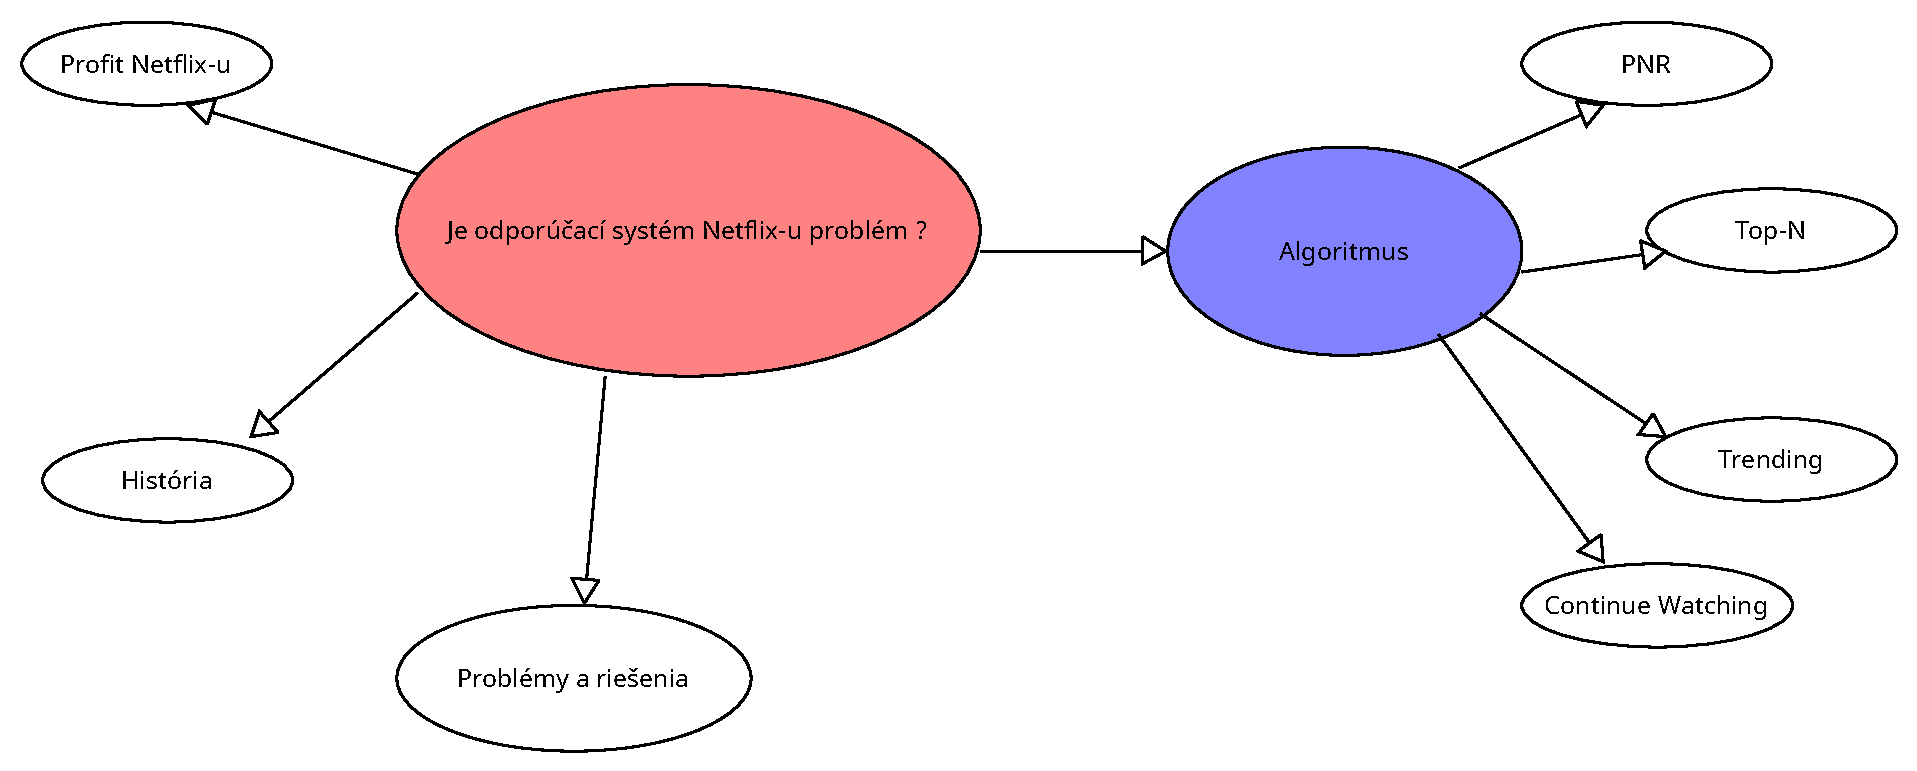
\includegraphics[scale=0.4]{UvodnyDiagram.pdf}
\end{figure}
\section{Krátka história} \label{Netflix cena} %viac o minulosti a o netflix prize
Už v roku 2006 mal Netflix záujem o odporúčacie systémy.\cite{amatriain2015recommender} Preto, oznámil Cenu Netflixu ako súťaž strojového učenia o to, kto vytvorí aspoň o 10\% lepší odporúčací systém ako bol ten ich, Cinematech. Nový odporúčací systém mal byť lepší v konkrétne \textit{RMSE(root mean squared error)}\footnote{RMSE - root mean squared error - odmocnina priemerného rozdielu medzi reálnymi a očakávanými hodnotami\cite{EncyclopaediaBritannica}} pre predpokladané hodnotenie. A zrazu sa veľmi veľa rozdielnych firiem snažilo zlepšiť svoje algoritmy.
%uz za tyzden ich prekonali, treba najst zdroj

\section{Problem zlatej rybky} \label{Krátka pozornosť}
Keď majú ľudia príliš veľa vecí, na ktoré sa môžu pozrieť, nepozrú sa na nič. Štúdia spomenutá v \cite{10.1145/2843948} zistila, že v priemere typický používateľ stráca pozornosť po pribižne minúte prezerania si možností, čo si pozrie. No a teda sa Netflix veľmi usiluje aby počas tejto minúty, ukázal užívateľovi čo najlepší výsledok. Určite sa aj vám niekedy stalo, že ste otvorili Netflix hlavnú stránku, chvíľku popozerali a potom Netflix vypli. To je pre Netflix najhoršia vec, čo môže nastať, pretože vy ste si nič nepozreli a aj napriek tomu, že im platíte mesačne, ak sa toto stane viac krát, určite to predplatné zrušíte. Nikto predsa nechce službu ktorá im neponúka to, čo chcú.

\section{Algoritmus} \label{Algoritmus}
Ak človek nemá žiadne odporúčanie od kamaráta alebo známeho, je odkázaný prehľadávať veľké množstvo filmov a seriálov, o ktorých nevieme či sú dobré alebo nie. Jednoducho si o každom z filmov alebo seriálov dokážeme dohľadať hodnotenia a žánre, ale nikdy nevieme, či sa to bude páčiť práve nám. A preto prichádzajú "na scénu", veľmi potrebné algoritmy ktoré vďaka veľkému množstvu dát dokážu predpovedať ako veľmi sa nám bude daná šou páčiť, ukázať nám hodnotenia ľudí podobnej filmovej chute ako my a dokonca aj predpovedať aké hodnotenie jej dáme. ''V Netflixe nieje jeden model ktorý poháňa všetky odporúčania ale skôr set techník ktoré sa navzájom prepájajú v rovnakom cieli - zvýšiť užívateľskú spokojnosť''\cite{Steck_Baltrunas_Elahi_Liang_Raimond_Basilico_2021}. No a teda aké všetky algoritmy vlaste používa Netflix na svojej platforme ? Viac sa dozviete v najbližších podkapitolách\ldots

\subsection{Prispôsobený hodnotič videí}
Na hlavnej stránke môžte vidieť naozaj veľa filmov a seriálov. Sú ale rozdelené do riadkov, vždy podľa toho čo ich spája. Pre uvedenie príkladu, riadok komediálnych filmov sa pre nás vytvorí, ak sme si niekedy predtým pozreli nejakú komédiu. Samozrejme sa to odvíja od toho, aký člen domácnosti práve pozerá, tak isto od toho aké hodnotenie dal danej komédií a tak isto ako dlho ju pozeral a koľko takých komédií si pozrel. Na všetkom z tohto pracuje \textit{PVR(Personalised Video Ranker)}\footnote{PVR - personal video ranker - Prispôsobený hodnotič videí\cite{10.1145/2843948}}\cite{10.1145/2843948}
\subsection{Top-N hodnotič videí}
Iný typ riadku ktorý je tiež na hlavnej stránke ale ukazuje trošku niečo iné. Jeho cieľ je taký istý - ukázať užívateľovi najlepší obsah. Pre zmenu, to teraz nefiltruje podľa iba určitého žánru ale z celého katalógu nám ukazuje to najlepšie čo bol schopný nájsť pre daného užívateľa a ukáže prvých 10, inokedy viac, odporúčaní, ktoré sú na začiatku ''listu'' ktoré vytvára tento algoritmus.\cite{amatriain2015recommender}
\subsection{Teraz populárne}
Tento algoritmus je veľmi jednoduchý aj naraz personalizuje aj ukazuje krátkodobo populárne filmy a seriály.
\subsection{Pokračujte v pozeraní}
Keďže je veľmi dôležité ukladať pokrok pozerania seriálov alebo filmov na pokračovanie, tento riadok je veľmi potrebný.


\section{Profitabilnosť} \label{Profit}

Keďže 80\% sledovania na platforme tvorí sledovanie odporúčaného obsahu práve predtým spomenutými algoritmami, tak to znamená, že fungujú veľmi dobre a, že sa im vyplatia \cite{pub.1158091188}. V podstate bez ohľadu na to, koľko by ich to stálo, vyplatí sa im udržiavať a vyvíjať tieto algoritmy. Keďže za prehrávanie určitého obsahu, či už populárneho a dobre hodnoteného alebo nepopulárneho a menej dobre hodnoteného, platí Netflix prakticky tú istú sumu a teda im je to v podstate jedno, čo užívateľovi zobrazí, jediné na čom záleží je, že si to užívateľ pozrie, je spokojný a príde na platformu znova. \cite{amatriain2015recommender}
Pre jednoduché porovnanie odporúčacieho systému Netflixu s napr. Spotify odporúčacím systémom. Môžme vidieť veľmi veľký problém v tom, že Spotify uprednostňuje populárnu hudbu a obsah oproti tomu menej populárnemu , pretože z toho má vačší profit a teda je stavaný aj ich odporúčací systém okolo profitu\cite{10425661}. Keďže každá firma chce mať profit, je to v relatívne v poriadku, ale problém je, že potom sú utláčaní nepopulárny umelci a majú ťažšie vytvoriť zisk. Na rozdiel od Spotify, Netflix profituje za všetok obsah rovnako, je menej podstatné uprednostňovať populárny obsah. O tom, že Netflix je na tom finančne veľmi dobre a raste aj nadalej oproti minulým rokom, hovorí aj ich výročná správa o profite\cite{AnnualReportNetflix2023}. Tento profit sa odvíja aj na hodnote ich akcie, tá bola v 01. novembra 2023 iba 420,19\$ ale tohto roka v ten istý dátum sa vyšplhala na neuveriteľných 756,10\$ za akciu. To je zvýšenie o takmer 80\% za jeden rok.\cite{StockValueNetflix}
%tabulka profitu potom porovnanie 2022 a 2023

\section{Rozloženie hlavnej stránky} \label{Rozloženie}
Keďže už sme si popísali ako fungujú algoritmy, teraz si môžme popísať ako personalizovaný obsah rozkladá na stránku. Ako už predtým bolo spomenuté, užívateľ má krátku dobu pozornosti a Netflix preto rozdeľuje tento obsah do riadkov hneď na hlavnú stránku. Treba si ale uvedomiť že Netflix je zväčša používaný v domácnostiach a teda do napr. top 10 sa snaží dávať obsah ktorý si užije napr. otec, mama a ďalší členovia rodiny. Tak isto sa snaží nájsť položku pre celú rodinu. Ak je rodina jednočlenná, tak sa snaží nájsť výber z rozdielnych nálad a záľub daného užívateľa ktoré zisťujú dané algoritmy.\cite{amatriain2015recommender}
Netflix chce aby sme vedeli, ako sa ich systém adaptuje našej chuti. To som si ale ja napríklad sám nevšimol\ldots A tak isto sa snaží vybudovať dôveru v tieto odporúčania a tiež sa snaží vysvetliť prečo by sme si to chceli pozrieť. Toto reprezentuje popisok k danemu filmu/serialu, tak isto to ukazuje predikciu hodnotenia ake by sme dali danému filmu/seriálu a tiež či si nejaky z našich priateľov pozrel daný obsah.


% \begin{figure}
% 	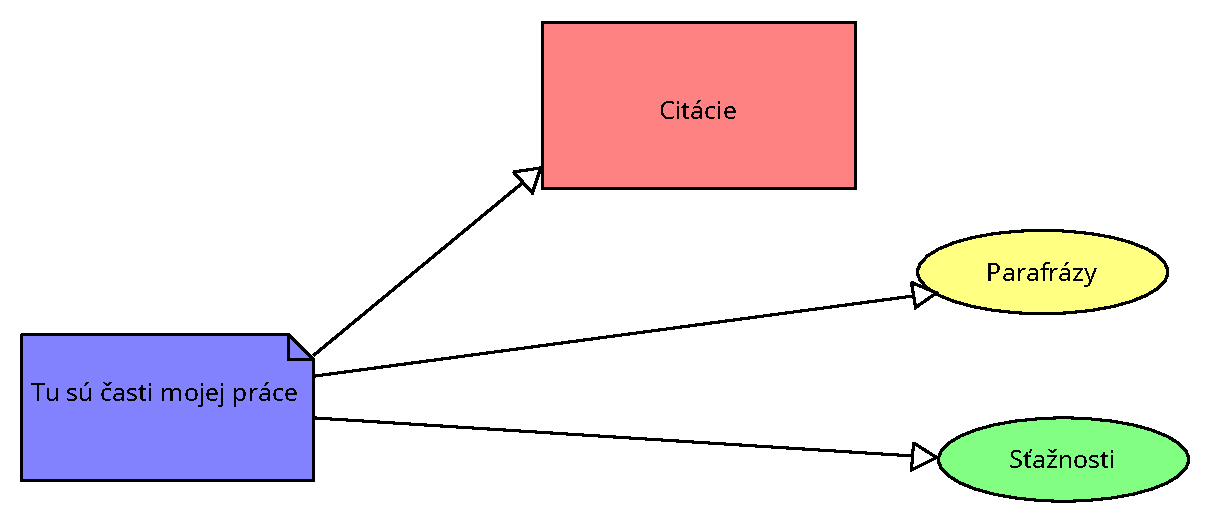
\includegraphics[scale=0.4]{diagram horizontal.pdf}
% \end{figure}



%\acknowledgement{Ak niekomu chcete poďakovať\ldots}


% týmto sa generuje zoznam literatúry z obsahu súboru literatura.bib podľa toho, na čo sa v článku odkazujete
%\begin{figure}
\bibliography{literatura}
\bibliographystyle{abbrv} % prípadne alpha, abbrv alebo hociktorý iný
%\end{figure}

\end{document}
